\chapter{Datenbank}
\newcounter{ids}

    \begin{figure}[h]
        \centering
        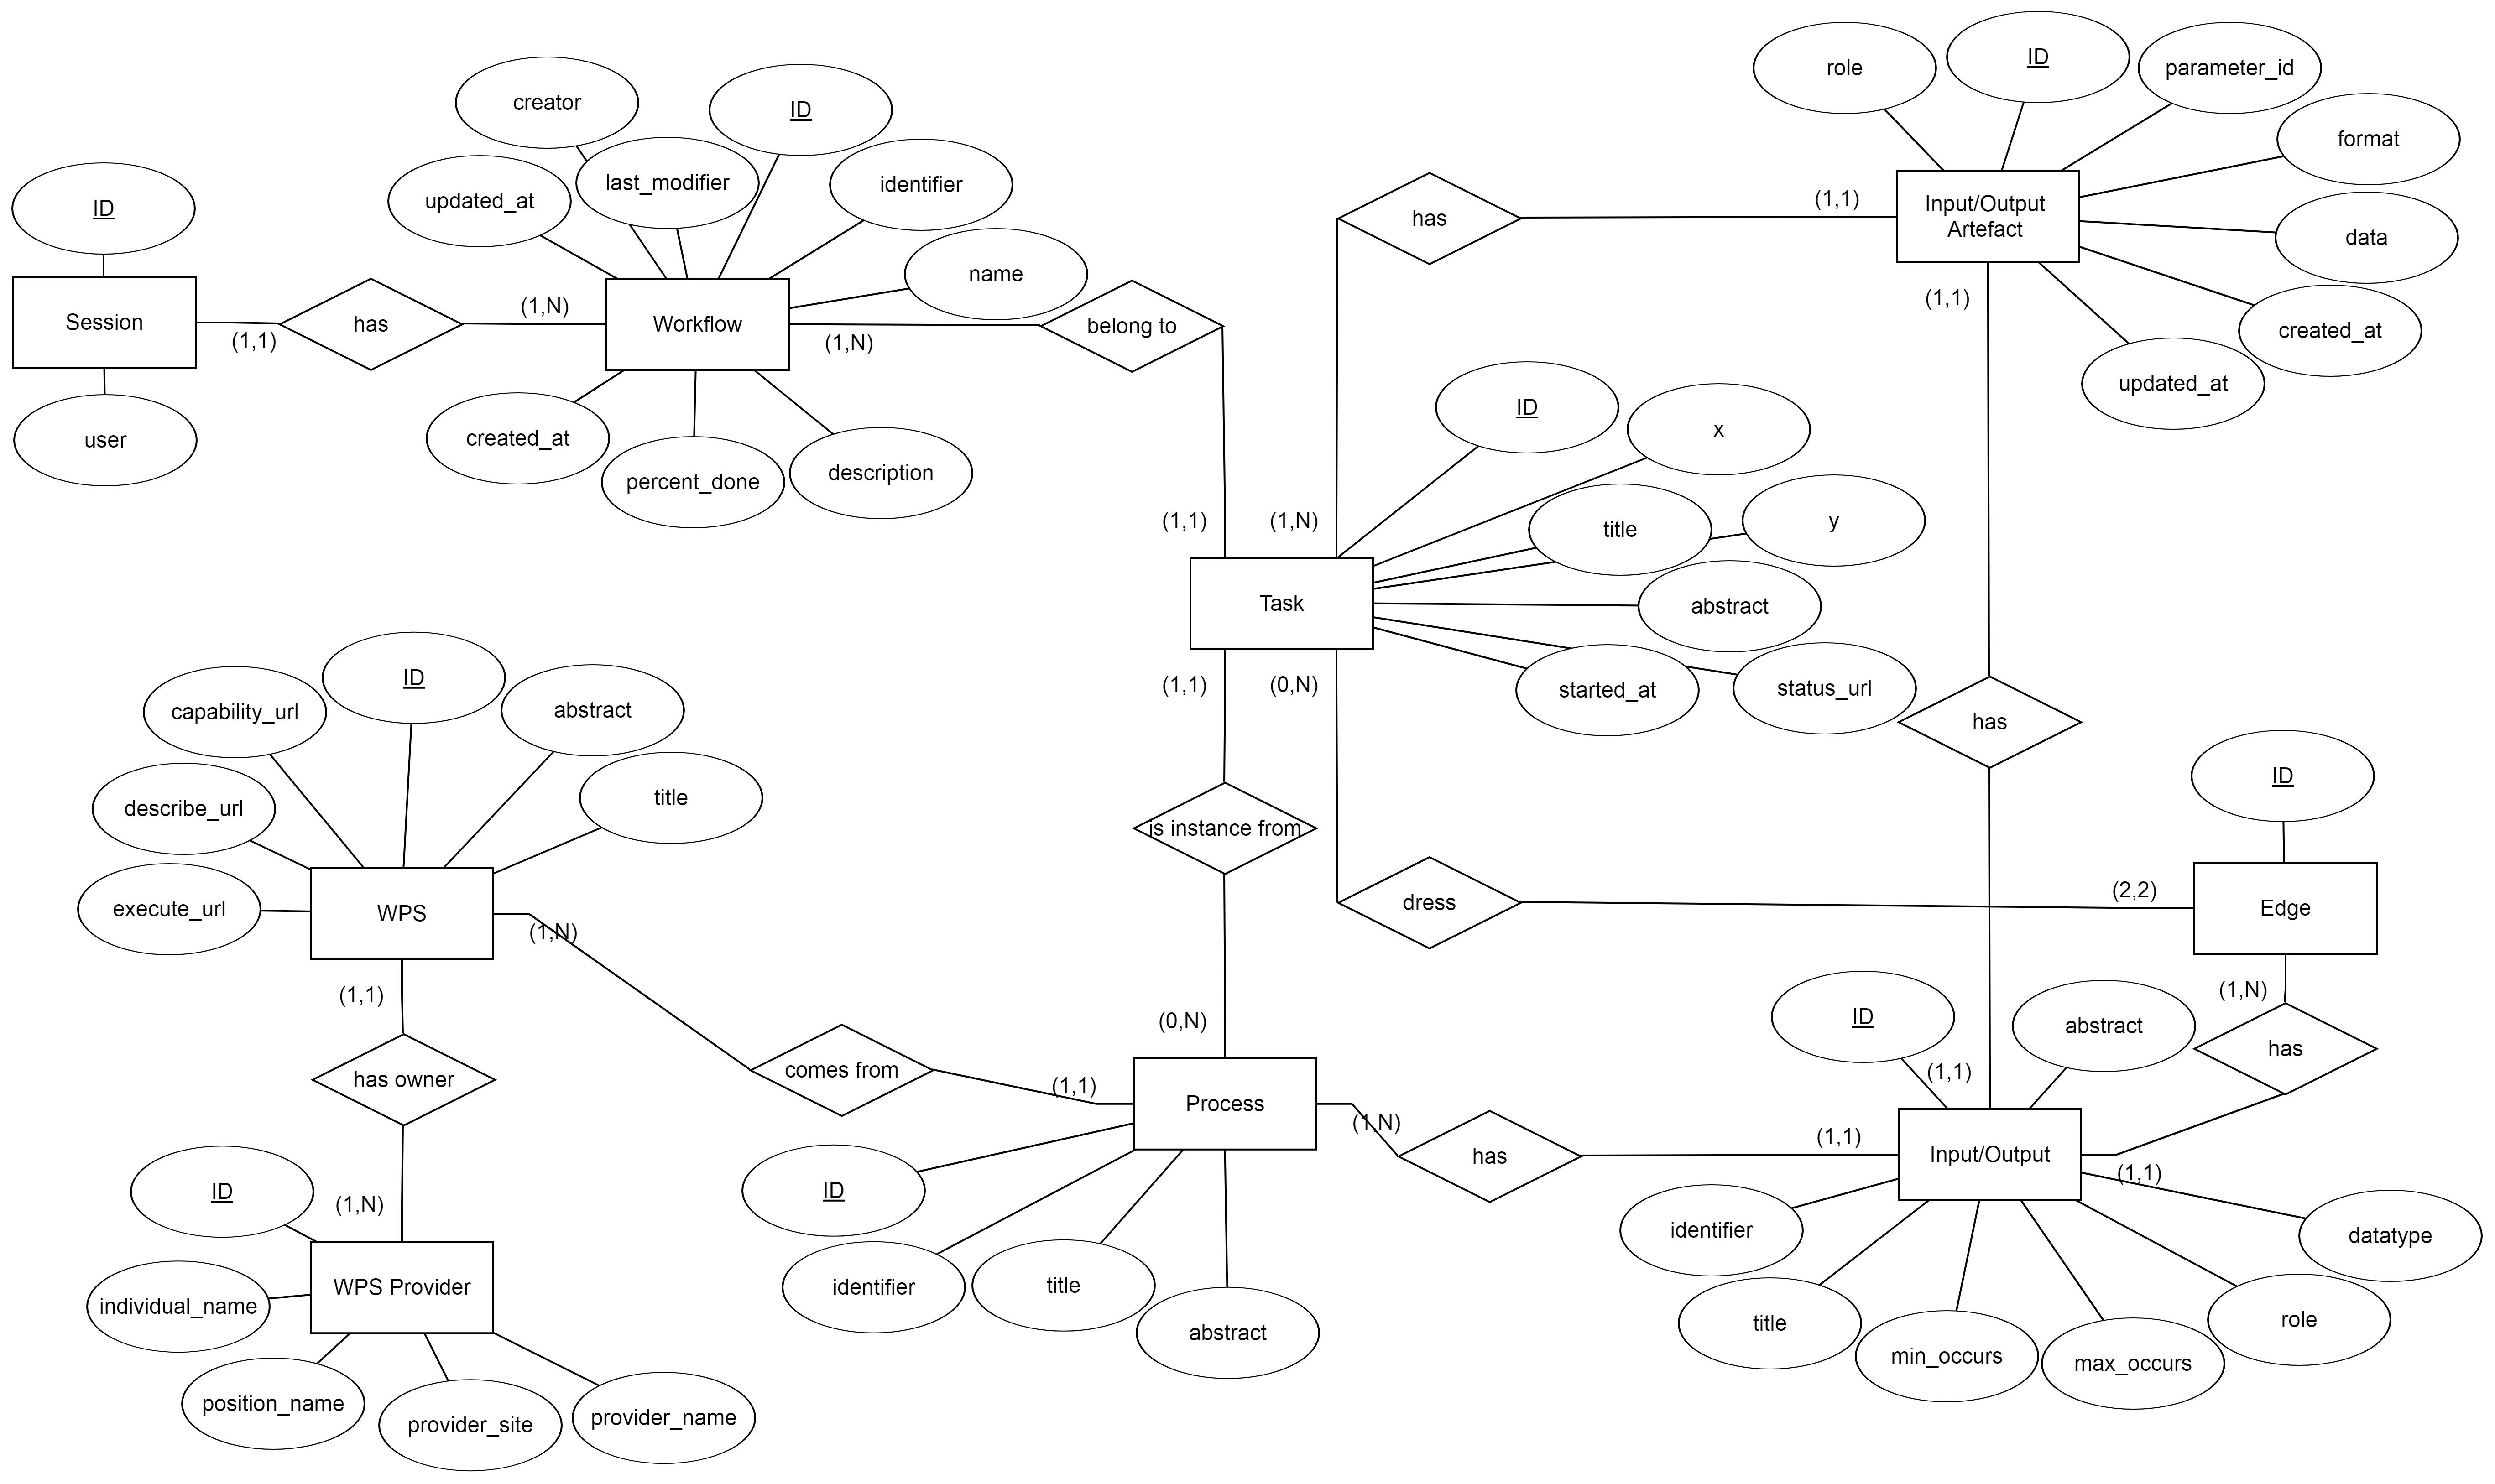
\includegraphics[width=15cm]{diagrams/ERDiagramm.png}
        \caption{Entity Relationship Diagram}
        \label{fig:er_diagramm}
    \end{figure}
    
    
	\section{Einleitung}
	
	hier kann sich jemand einen schönen text für ausdenken...
	
	
	\section{Tabellen}
	
 		\subsection{Session}
 		\begin{center}
 			\setlength\tabcolsep{5pt}
 			\renewcommand{\arraystretch}{1.5}
 			\setcounter{ids}{0}			
 			\begin{tabular}{|c|c|c|}
 				\hline
 				\rowcolor[gray]{0.75}[4.85pt]
 				id & user & last\_workflow \\ \hline  
 				\stepcounter{ids}\arabic{ids} & & \\	
 				\hline
 			\end{tabular}
 		\end{center}		


 		\subsection{WPSProvider}
 		\begin{center}
 			\setlength\tabcolsep{5pt}
 			\renewcommand{\arraystretch}{1.5}
 			\setcounter{ids}{0}			
 			\begin{tabular}{|c|c|c|c|c|}
 				\hline
 				\rowcolor[gray]{0.75}[4.85pt]
 				id & provider\_name & provider\_site & individual\_name & position\_name \\ \hline  
 				\stepcounter{ids}\arabic{ids} & &&& \\	
 				\hline
 			\end{tabular}
 		\end{center}		


		\subsection{Edge}
		\begin{center}
			\setlength\tabcolsep{5pt}
			\renewcommand{\arraystretch}{1.5}
			\setcounter{ids}{0}			
			\begin{tabular}{|c|c|c|c|c|c|}
				\hline
				\rowcolor[gray]{0.75}[4.85pt]
				id & workflow & from\_task & to\_task & input & output \\ \hline  
				\stepcounter{ids}\arabic{ids} & &&&& \\	
				\hline
			\end{tabular}
		\end{center}		
		
		\subsection{Process}
		\begin{center}
			\setlength\tabcolsep{5pt}
			\renewcommand{\arraystretch}{1.5}
			\setcounter{ids}{0}			
			\begin{tabular}{|c|c|c|c|c|}
				\hline
				\rowcolor[gray]{0.75}[4.85pt]
				id & wps & identifier & title & abstract \\ \hline  
				\stepcounter{ids}\arabic{ids} & &&& \\	
				\hline
			\end{tabular}
		\end{center}		
		

		\subsection{WPS}   
		\begin{center}
			\setlength\tabcolsep{5pt}
			\renewcommand{\arraystretch}{1.5}
			\setcounter{ids}{0}			
			\begin{tabular}{|c|c|c|c|c|c|c|}
				\hline
				\rowcolor[gray]{0.75}[4.85pt]
				id & service\_provider & title & capabilities\_url & describe\_url & execute\_url & abstract \\ \hline
				&&&&&& \\
				\hline
			\end{tabular}
		\end{center}

		\subsection{Task}
		\begin{center}
			\setlength\tabcolsep{5pt}
			\renewcommand{\arraystretch}{1.5}
			\setcounter{ids}{0}			
			\begin{tabular}{|c|c|c|c|c|c|c|c|c|c|}
				\hline
				\rowcolor[gray]{0.75}[4.85pt]
				id & workflow & process & x & y & status & title & status\_url & started\_at & abstract \\ \hline  
				&&&&&&&&& \\
				\hline
			\end{tabular}
		\end{center} 
		
		
		\subsection{Workflow}
		\begin{center}
			\setlength\tabcolsep{5pt}
			\renewcommand{\arraystretch}{1.5}
			\setcounter{ids}{0}			
			\begin{tabular}{|c|c|c|c|c|c|c|c|}
				\hline
				\rowcolor[gray]{0.75}[4.85pt]
				id & name & percent\_done & created\_at & update\_at & creator & last\_modified & description \\ \hline 
				&&&&&&& \\
				\hline
			\end{tabular}
		\end{center}
		
		
		
		\subsection{InputOutput}
		\begin{center}
			\setlength\tabcolsep{5pt}
			\renewcommand{\arraystretch}{1.5}
			\setcounter{ids}{0}			
			\begin{tabular}{|c|c|c|c|c|c|c|c|c|}
				\hline
				\rowcolor[gray]{0.75}[4.85pt]
				id & process & role & identifier & title & datatype & min\_occurs & max\_occurs & abstract \\ \hline 
				&&&&&&&& \\
				\hline
			\end{tabular}
		\end{center}
		
		
		\subsection{Artefact}
		\begin{center}
			\setlength\tabcolsep{5pt}
			\renewcommand{\arraystretch}{1.5}
			\setcounter{ids}{0}			
			\begin{tabular}{|c|c|c|c|c|c|c|c|}
				\hline
				\rowcolor[gray]{0.75}[4.85pt]
				id & task & parameter & role & format & data & created\_at & updated\_at \\ \hline 
				&&&&&&& \\
				\hline
			\end{tabular}
		\end{center}		
		
		
%	
%		
%		\newpage
%		
%		\paperwidth=\pdfpageheight
%		\paperheight=\pdfpagewidth
%		\pdfpageheight=\paperheight
%		\pdfpagewidth=\paperwidth
%		\headwidth=1.05\textheight
%		
%		\begingroup 
%		\vsize=\textwidth
%		\hsize=1.05\textheight
%		
%		\textwidth=\hsize
%		\textheight=\vsize
%
%	
%		
%
%			
%			
%		
%		
%		
%	\endgroup
%	\newpage
%	\paperwidth=\pdfpageheight
%	\paperheight=\pdfpagewidth
%	\pdfpageheight=\paperheight
%	\pdfpagewidth=\paperwidth
%	\headwidth=\textwidth
	
        
    \section{Kommunikationsmodell}
	    
	    hier schemazeichnung von den komponenten (servern, etc) und pfeile mit kommunikationsrichtung, um datenverkehr darzustellen. daraus soll hervorgehen, dass datenbank das datenkonsistenzglied ist
	    